%% This is an example first chapter.  You should put chapter/appendix that you
%% write into a separate file, and add a line \include{yourfilename} to
%% main.tex, where `yourfilename.tex' is the name of the chapter/appendix file.
%% You can process specific files by typing their names in at the 
%% \files=
%% prompt when you run the file main.tex through LaTeX.
\chapter{Results and Testing}
This chapter will describe 
\section{An Example: String Quartet No.7 in E-flat major, K.160}
This section will walk through an example of how the entire \texttt{OMRMIDICorrector} system works on Mozart's \textit{String Quartet No.7 in E-flat major, K.160}.

\subsection{Preparing the Raw Input}
The basic raw input of the system is an OMR score and a MIDI file. A scanned copy of the score was found in IMSLP \cite{k160}, the source for much free public domain sheet music. The MIDI file was sourced from the Yale MIDI Archive\cite{yalemidiarchive}, whose contents are now hosted on MuseData \cite{musedata}. [[double check this with Myke]]

I prepped the pdf score using SmartScore X2 Pro, splitting the pdf into its three movements and cropping out extraneous information in the title portion of the page. Then I ran the cropped movements through SmartScore's built-in OMR tool (It is important to note that while SmartScore is proprietary, there is also free and open source software that also has OMR tools). Then I saved the post-OMR file as a musicXML file. 

\begin{figure}[!ht]
\centering
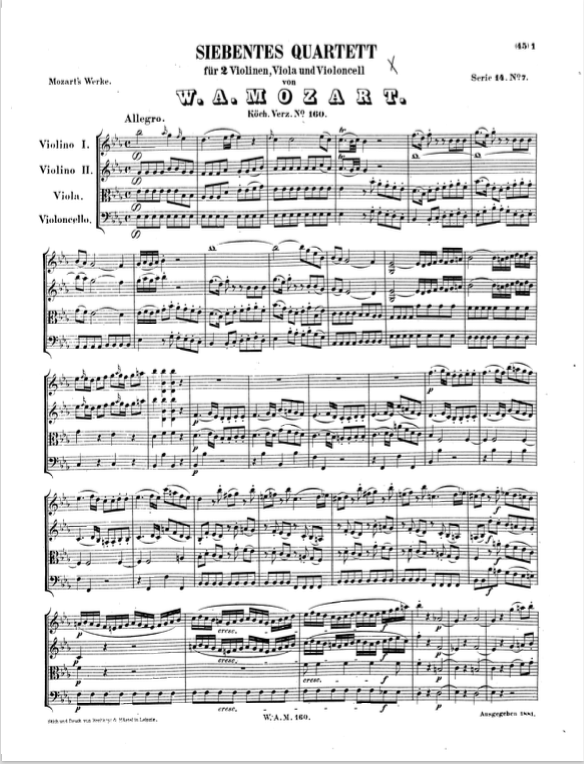
\includegraphics[width =.6\textwidth]{k160uncroppedfirstpage}
\caption{The uncropped first page of k160 contains extraneous noise in the title section.}
\end{figure}

I prepped the MIDI file by opening it in SmartScore X2 Pro and saving as a musicXML file (It is important to note that while SmartScore is proprietary, there is also free and open source software that also converts .mid files to musicXML files).

The last step of preparing the raw input is to parse the musicXML files with the \texttt{music21} library so that they are \texttt{Stream} objects. This can be done by passing in the musicXML filepaths to the \texttt{parse} method in the \texttt{converter} class. We will call these two parsed streams \texttt{midiStream} and \texttt{omrStream}. 

\section{Existing Music}
\section{Timing} \label{timing}

